\part{Operating System}

\chapter{Introduction}
\section{An Introduction to Operating System}
\subsection{OS and its functionalities}
\paragraph{What is OS}?
\begin{itemize}
	\item \textbf{Definition-1:} It's a program that lets you run other programs. We need to differentiate this from a command interpreter or a windowing system, which run other programs based on user requests.
	\item \textbf{Definition-2:} A program that provides controlled access to a computer's resources. These resources include the CPU (process scheduling), memory (memory management), display, keyboard, mouse (device drivers), persistent storage (file systems) and the network.
\end{itemize}
\subsubsection{What are the functions of OS?}
\subsection{Different Types of OS}
\subsubsection{Batch Processing Operating System} 
\begin{itemize}
	\item Many programs with similar requirements are added to the system in bunch
	\item Only one Job can run at a time serially
	\item Reduced CPU utilization
\end{itemize}

\subsubsection{Multi-Programming Operating System}
\begin{itemize}
	\item Multiple programs resides in main memory
	\item if n nos. of processes are in main memory then n is called degree of multi-programming,
	\item degree of multi-programming doesn't depend of number of CPUs.
	\item have better CPU utilization and throughput
\end{itemize}
\subsubsection{Multi-Tasking Operating System}
\begin{itemize}
	\item logical extension of multi-programming systems
	\item jobs are executed on the CPU in time sharing mode
	\item added advantage of better response time
\end{itemize}
\subsubsection{Multi-Threading Operating System}
\subsubsection{Multi-Processing Operating System}
\subsubsection{Real-time Operating System}
\begin{itemize}
	\item Each process must finished within well defined fixed time
	\begin{enumerate}
		\item \textbf{Hard Real-time System}
		\item \textbf{Soft Real-time System}
	\end{enumerate}
\end{itemize}
\subsubsection{Distributed Operating System}
\begin{itemize}
	\item 
	\item Also known as loosely coupled system
\end{itemize}
\section{Kernel}
\subsection{System Calls}
System calls provide an interface to the services made available by an operating system. Usually invoked by software interrupt.
\begin{center}
	\begin{tabular}{| l | c | c |}
		\hline \textbf{Categories} & \textbf{WINDOWS} & \textbf{UNIX}  \\
		\hline \multirow{3}{7em}{Process Control} & CreateProcess() & fork()\\
		& ExitProcess() & exit()\\
		& WaitForSingleObject()& wait() \\ 
		\hline \multirow{3}{7em}{File Manipulation} & CreateFile() & open()\\
		& ReadFile() & read()\\
		& WriteFile() & write() \\
		& CloseHandle() & close()\\
		\hline \multirow{3}{7em}{Information Maintenance} & GetCurrentProcessID() & getpid()\\
		& SetTimer() & alarm()\\
		& Sleep()& sleep() \\
		\hline \multirow{3}{7em}{Device Manipulation} & SetConsoleMode() & ioctl()\\
		& ReadConsole() & read()\\
		& WriteConsole()& write() \\
		\hline \multirow{3}{7em} {Communication} & CreatePipe() & pipe()\\
		& CreateFileMapping() & shmget()\\
		& MapViewOfFile() & mmap()\\
		\hline \multirow{3}{7em}{Protection} & SetFileSecurity() & chmod()\\
		& InitializeSecurityDescriptor() & umask()\\
		& SetSecurityDescriptorGroup() & chown()\\
		\hline   
	\end{tabular}
\end{center}
\paragraph{fork()}
\begin{itemize}
	\item Mainly used for creating child process
	\item return 0 to child and a non zero value to parent on success
	\item return -ve value on failure
	\item If the program contains 'n' fork () system calls, then Number of child processes created = 2n–1.
\end{itemize}

\chapter{Process Management}
\section{Process Concept}
\subsection{Process Lifecycle}
\subsubsection{Process States}
\begin{itemize}
	\item \textbf{Created} Process is newly created by system call, is not ready to run.
	\item \textbf{Running} Only One process can be in running state.
	\item \textbf{User running} Process is running in user mode which means it is a user process.
	\item \textbf{Kernel Running} Indicates process is a kernel process running in kernel mode.
	\item \textbf{Zombie} Process does not exist/ is terminated.
	\item \textbf{Preempted} When process runs from kernel to user mode, it is said to be preempted.
	\item \textbf{Ready to run in memory} It indicated that process has reached a state where it is ready to run in memory and is waiting for kernel to schedule it.
	\item \textbf{Ready to run, swapped–} Process is ready to run but no empty main memory is present
	\item \textbf{Sleep, swapped} Process has been swapped to secondary storage and is at a blocked state.
	\item \textbf{Asleep in memory} Process is in memory(not swapped to secondary storage) but is in blocked state.
\end{itemize}
\begin{figure}[H]
	\centering
	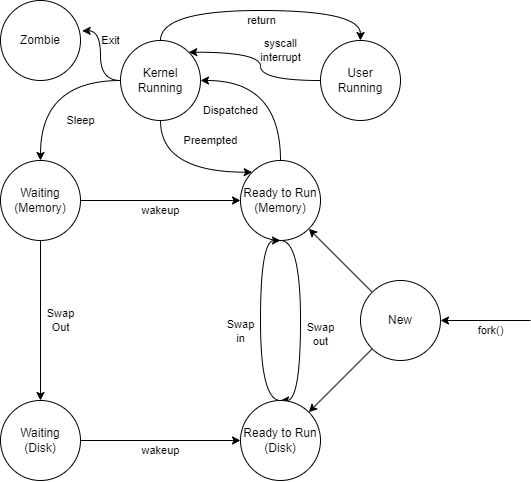
\includegraphics[width=\textwidth]{process_state}
	\caption{Process State Transition}\label{fig_process_state_diagram}
\end{figure}
\subsection{Process Control}
\subsubsection{Process Control Block}
\paragraph{Structure of Process Control Block}
\begin{enumerate}
	\item Process State: created, ready to run, run, asleep, zombie, preempted, orphan etc.
	\item PID: Unique ID of the process
	\item Program Counter: Address of the next instruction
	\item Registers: Stack Pointers, Index Registers etc.
	\item Memory Management Information: Paging, Segmentation etc.
	\item Scheduling Info: Priority of processes, the implemented algorithms etc. 
	\item Open file lists: The resources that are in use devices, files etc.
	\item Timing Info: Running time, Remaining CPU burst, CPU utilization.
\end{enumerate}
\paragraph{Some notable points}
\begin{itemize}
	\item implemented using \textbf{double linked list}
	\item each process has it's own PCB
	\item PCB of all processes stored in \textbf{main memory}
\end{itemize}

\subsection{Process Modes}
The primary goal of the dual mode operation is to provide protection and security to the user application programs and the
operating system from the unauthorized users. The mode bit is used to determine the particular mode in which an instruction
is executing.
\subsubsection{User Mode}
\begin{itemize}
	\item direct access to the hardware 
	\item full access to the machine instruction set
	\item I/O operations, context-switching, clearing the memory map
\end{itemize}

\subsubsection{Kernel Mode}
\begin{itemize}
	\item direct access to the hardware 
	\item full access to the machine instruction set
	\item I/O operations, context-switching, clearing the memory map
\end{itemize}

\subsubsection{Mode Switching} Steps involving switching between kernel mode and user mode\\
\begin{tabular}{|l|l|}
	\hline 
	Mode bit: 0 & Kernel mode \\ 
	\hline 
	Mode bit: 1 & User mode \\ 
	\hline 
\end{tabular} 

\subsection{Context}
\subsubsection{Context Switching}
\paragraph{What is Context Switching?}
A context switch is storing the state or context of a process so that it can be reloaded whenever required for execution from the same point it was switched as earlier. Context switches can occur only in kernel mode.
\subparagraph{The steps of context switching}
A typical thread context switch on a CPU happens like this:
\begin{enumerate}
	\item Save the context of the process that is currently running on the CPU.
	\item Update the process control block and other important fields.
	\item Move the process control block of the above process into the relevant queue such as the ready queue, I/O queue etc.
	\item Select a new process for execution.
	\item Update the process control block of the selected process. This includes updating the process state to running.
	\item Update the memory management data structures as required.
	\item Restore the context of the previous process by loading the old values of the process control block and registers loaded again on the processor
\end{enumerate}

\section{Process Scheduling}
\subsection{Process Schedulers}
\paragraph{Short Term Schedulers} Select a job from ready queue based on its policy and gives the control of the CPU to that process with the help of "Dispatcher". Also known as CPU scheduler.
\begin{itemize}
	\item $Ready \rightarrow Run$
\end{itemize}
\paragraph{Mid Term Schedulers} If a process requests an I/O in the middle of execution, then the process removed from the main memory is loaded into the waiting queue of secondary memory (\textbf{swap-out}). When the I/O operation is completed, then the job moved from waiting queue of secondary memory to ready queue (\textbf{swap-in}). Also known as swapper.
\begin{itemize}
	\item $Ready \leftrightarrow Suspend Ready$
	\item $Block \leftrightarrow Suspend Block$
\end{itemize}
\paragraph{Long Term Schedulers} Select a job from disk and decides whether it should load it into main memory or not. Choosing a good mix of CPU/IO bound processes is main task. Also known as job Scheduler.
\begin{itemize}
	\item $New \rightarrow Ready$
\end{itemize}
\paragraph{Dispatcher}
\begin{itemize}
	\item loading the job onto the CPU
	\item perform context-switching
\end{itemize}
\begin{figure}[H]
	\centering
	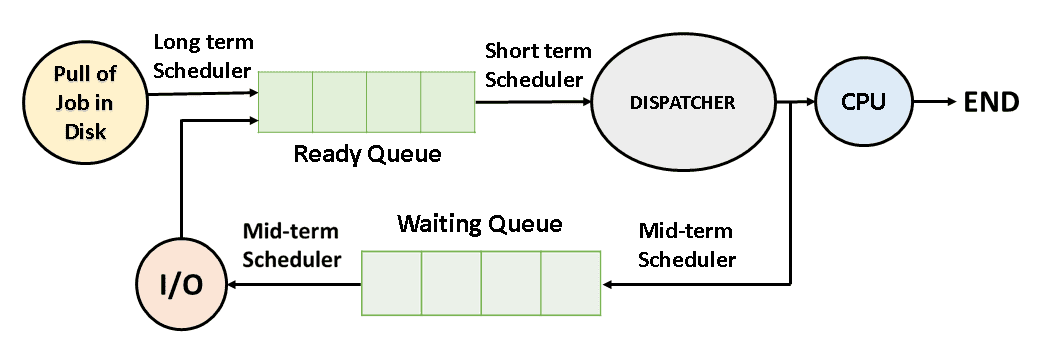
\includegraphics[width=\textwidth]{process_scheduler}
	\caption{Process Schedulers}\label{fig_process_scheduler_diagram}
\end{figure}

\subsection{CPU Scheduling Criteria} CPU Scheduling Criteria in OS
\paragraph{CPU Utilization $(\uparrow)$} This is the percentage of time that the processor is busy, CPU utilization may range from 0-100\%.
\paragraph{Throughput $(\uparrow)$} It means how many jobs are completed by the CPU.
\paragraph{Waiting Time $(\downarrow)$} Waiting time is the sum of the periods spent waiting by a process in the ready queue.
\paragraph{Response Time $(\downarrow)$} Response time is the time duration between the submission and the first response.
\paragraph{Turnaround Time} The time interval between the submission of the process and the time of the completion is the turnaround time. This is the turnaround time formula in OS [Turnaround time = Waiting time in the ready queue + executing time + waiting time in waiting-queue for I/O].
\paragraph{Arrival Time} time required from birth to the Ready state
\paragraph{Burst / Service Time} time required by the process to complete execution

\subsection{Process Scheduling Algorithms}
\paragraph{First Come First Serve (FCFS)}
\begin{itemize}
	\item This is a non-preemptive algorithm
	\item Use queue (FIFO) for implementation
    \item Free from Starvation
    \item Suffers from \textit{convoy effect}
\end{itemize}
\paragraph{Last Come First Serve (LCFS)}
\begin{itemize}
	\item This is a non-preemptive algorithm
	\item Use stack (LIFO) for implementation
\end{itemize}
\paragraph{Priority Based}
\begin{itemize}
    \item May be preemptive or non-preemptive
	\item Suitable for realtime systems where critical task to be finished first and deadline to be met
\end{itemize}
\paragraph{Shortest Job First (SJF)}
\begin{itemize}
	\item non-pre-emptive algorithm.
    \item Extension of priority scheduler, here highest priority is given to the process with smallest CPU burst time
    \item Large processes may starve
    \item CPU burst time is unknown at the time of arrival
    \item Minimizes average response time of processes
\end{itemize}
\paragraph{Shortest Remaining Task First (SRTF)}
\begin{itemize}
	\item preemptive algorithm
    \item shortest job at this instant is assigned to the CPU
    \item Large processes may starve
    \item Minimizes the average turnaround time of the processes
\end{itemize}
\paragraph{Round-Robin (RR)}
\begin{itemize}
	\item preemptive algorithm. 
	\item CPU has a fixed time quantum i.e. each Process is given a limited time to complete its task. If it gets completed within that fixed time or the time is over then the control of CPU is given to another process waiting in the queue. Creates a illusion that all processes is running at the same time.
	\item Used mainly in time-sharing systems.
	\item $ns + (n-1)q = t$ where n is number of jobs, s is process switching time, q is time quantum
\end{itemize}
\paragraph{Highest Response Ratio Scheduling (HRRS)}
\begin{itemize}
    \item non-preemptive algorithm.
    \item No starvation
    \item Processes are assigned to the CPU based on their highest response ratio
    \item $ResponseRatio=\frac{WT+BT}{BT}$, Favors jobs that are waiting longer    
    
\end{itemize}
\paragraph{Multilevel Queue}
\begin{itemize}
	\item Used both priority and round-robin scheduling
    \item Processes are put into multiple levels based on priority
    \item multiple processes in the highest-priority queue, are executed in round-robin order
    \item Common division Foreground Process (Realtime process, System process, interactive process), Background Process (batch process)
\end{itemize}
\paragraph{Multilevel Feedback Queue}
\begin{itemize}
	\item Processes moves between queue
    \item I/O-bound \& interactive processes which are typically characterized by short CPU bursts are put in the higher-priority queues if a process uses too much CPU time that demoted to low priority queue
\end{itemize}
\begin{table}[H]
	\begin{center}
		\begin{tabular}{|l|c|c|c|c|}
			\hline
			\rowcolor{gray!20}
			\thead{Scheduling Algorithm} & \thead{CPU Overhead} & \thead{Throughput} & \thead{TAT} & \thead{RT} \\
			\hline
			FIFO & LOW & LOW & HIGH & LOW \\
			\hline
			SJF & MEDIUM & HIGH & MEDIUM & MEDIUM \\
			\hline
			PRIORITY & MEDIUM & LOW & HIGH & HIGH \\
			\hline
			ROUND ROBIN & HIGH & MEDIUM & MEDIUM & HIGH \\
			\hline
		\end{tabular}
		\caption{Comparison between different scheduling}
		\label{tbl-scheduling-comparison}
	\end{center}
\end{table}

\section{Threading}
\subsection{Threading Concept}
\subsection{Thread Control Block}
\begin{itemize}
	\item \textbf{Thread ID} Unique ID for each thread.
	\item \textbf{Thread states} Current state of the thread
	\item \textbf{CPU information} Program Counters and Registers
	\item \textbf{Thread Priority} Priority of that thread
	\item A pointer which points to the process which triggered the creation of this thread.
	\item A pointer which points to the thread(s) created by this thread.
\end{itemize}
\subsection{Thread Types}
\subsubsection{Based on level}
\paragraph{Kernel level threads}
\begin{itemize}
	\item Kernel level threads are supported and managed directly by the operating system.
	\item The kernel knows about and manages all threads.
	\item One process control block (PCP) per process.
	\item One thread control block (TCB) per thread in the system.
	\item Provide system calls to create and manage threads from user space.
\end{itemize}

\subparagraph{Advantages}
\begin{itemize}
	\item The kernel has full knowledge of all threads.
	\item Scheduler may decide to give more CPU time to a process having a large number of threads.
	\item Good for applications that frequently block.
	\item The context size is more
	\item Hardware support is required
\end{itemize}

\subparagraph{Disadvantages}
\begin{itemize}
	\item Kernel manage and schedule all threads.
	\item Significant overhead and increase in kernel complexity.
	\item Kernel level threads are slow and inefficient compared to user level threads.
	\item Thread operations are hundreds of times slower compared to user-level threads.
\end{itemize}

\paragraph{User level threads}
\begin{itemize}
	\item User level threads are supported above the kernel in user space and are managed without kernel support.
	\item Threads managed entirely by the run-time system (user-level library).
	\item Ideally, thread operations should be as fast as a function call.
	\item The kernel knows nothing about user-level threads and manage them as if they where single-threaded processes.
	\item The context size is less
	\item No hardware support required
\end{itemize}

\subparagraph{Advantages}
\begin{itemize}
	\item Can be implemented on an OS that does not support kernel-level threads.
	\item Does not require modifications of the OS.
	\item Simple representation: PC, registers, stack and small thread control block all stored in the user-level process address space.
	\item Simple management: Creating, switching and synchronizing threads done in user-space without kernel intervention.
	\item Fast and efficient: switching threads not much more expensive than a function call.
\end{itemize}
\subparagraph{Disadvantages}
\begin{itemize}
	\item Not a perfect solution (a trade off).
	\item Lack of coordination between the user-level thread manager and the kernel.
	\item OS may make poor decisions like:
	\begin{itemize}
		\item scheduling a process with idle threads
		\item blocking a process due to a blocking thread even though the process has other threads that can run
		\item giving a process as a whole one time slice irrespective of whether the process has 1 or 1000 threads
		\item unschedule a process with a thread holding a lock.
	\end{itemize}
	\item May require communication between the kernel and the user-level thread manager (scheduler activation) to overcome the above problems.
\end{itemize}
\subsubsection{Based on Number}
\paragraph{Single-threading}
\paragraph{Multi-threading}
\subparagraph{Multi-Threading Model}
\begin{itemize}
	\item \textbf{One-to-One} Each user level thread is mapped to single kernel-level thread
	\item \textbf{Many-to-One} Many user level threads are mapped to single kernel-level thread.
	\item \textbf{Many-to-Many} Many user level threads are mapped to multiple kernel-level threads
\end{itemize}
\subparagraph{Disadvantages}
\begin{itemize}
	\item Blocking one user-level thread of a process blocks the entire process
	\item TCB is considered as overhead for the system
\end{itemize}
\section{Process Coordination}
\subsection{Process Communication}
\subsubsection{Types of Communication}
\begin{itemize}
	\item \textbf{Cooperative} Execution of one process affects or affected by other process
	\item \textbf{Independent} No communication between processes
\end{itemize}
\subsection{Problems arises for not having synchronization}
\subsubsection{Producer Consumer} %TBD
\subsubsection{Dining Philosopher Problem} %TBD
\subsection{Synchronization}
\subsubsection{Critical Section}
\begin{itemize}
	\item \textbf{Critical Section} The portion of program text where shared variables or shared resources will be placed.
	\item \textbf{Non-Critical Section} The portion of program text where the independent code of the processes will be placed.
	\item \textbf{Race condition} The final value of any variable depends on execution sequence of the processes in which access takes place.
	\item To avoid the Race condition, only one process is allowed to enter into critical section
\end{itemize}
\paragraph{Conditions for handling critical Section}
To prove that this solution is correct. All the following conditions to be satisfied. 
\begin{itemize}
	\item \textbf{Mutual Exclusion} Only one process is allowed to enter into critical section at any point of time
	\item \textbf{Progress} No process that are running in remainder section can choose who can run in the critical section. Selection cannot be postponed indefinitely
	\item \textbf{Bounded Waiting} No process should have to wait forever to enter into critical section, there should be a bound/limit or it will lead to starvation.
\end{itemize}
\subsubsection{Solutions for Critical Section Problem}
\paragraph{Peterson’s solution}
\begin{itemize}
    \item Classic Software based solution
    \item May or may not work on RISC systems    
    \item every processes given a number i
    \item the turn indicates which process's turn to enter into critical section
    \item flag indicates if a process want to enter in critical section
    \item always gives way to the other process
\end{itemize}
\begin{lstlisting}
    boolean flag[2];
    while (true) {
        flag[i] = true;
        turn = j;
        while (flag[j] && turn == j);
        /* critical section */
        flag[i] = false;
        /* remainder section */
    }
\end{lstlisting}

\begin{tabular}{|c|c|c|c|}
    \hline
    \thead{Algorithm Name} & \thead{Mutual Exclusion} & \thead{Progress} & \thead{Bounded Waiting} \\
    \hline
    Lock Variable & $\times$ & $\surd$ & $\times$ \\
    \hline
    Decker’s Algorithm & $\surd$ & $\times$ & $\surd$ \\
    \hline
    Peterson’s Algorithm & $\surd$ & $\surd$ & $\surd$ \\
    \hline
    TSL Instruction & $\surd$ & $\surd$ & $\times$ \\
    \hline
\end{tabular}
\subsubsection{Monitor}
\begin{itemize}
    \item Monitors is a programming language compiler support type of solution to achieve synchronization.
    \item Monitors is collection of variables and procedures combined together in a special kind of module or package.
    \item The process running outside the monitor cannot directly access the internal variables of the monitor but however they can call the procedures of the monitor.
    \item Monitors has an important property that only one process can be active inside the monitor at any point of time.
\end{itemize}
\subsubsection{Semaphore}
Semaphore is an integer variable which is used by the various processes in a mutual exclusive manner to achieve synchronization.
\begin{itemize}
    \item Down(); or wait (); or p ()
    \item up(); or signal (); or v (); or release ();
\end{itemize}
\paragraph{Binary Semaphore}
\paragraph{Counting Semaphore}

\subsection{Deadlock}
\subsubsection{Deadlock Characteristics}
\begin{itemize}
	\item \textbf{Mutual Exclusion} Each resource can be assigned to at most one process only.
	\item \textbf{Hold and Wait} Processes hold a resource and may seek an additional resource.
	\item \textbf{No Preemption} Processes that have been given a resource cannot be preempted to release their resources.
	\item \textbf{Circular Wait} Every process awaits release of at least one resource held by some other processes.
\end{itemize}

A deadlock can occur only when all four conditions are present simultaneously.
\subsubsection{Deadlock Prevention}
\paragraph{Methods for deadlock prevention}
Deadlock can be prevented by unsatisfying one of the deadlock characteristics
\begin{itemize}
    \item \textbf{Mutual Exclusion} cannot be unsatisfied because of the concept of sharable and non-sharable resources
    \item \textbf{Hold and Wait}
    \begin{itemize}
        \item A process should be assigned all the required resources before the start of its execution. This may lead to low device utilization
        \item The process should release all the existing resources before making a new request. This may eventually lead to starvation.
    \end{itemize}
    \item \textbf{No Preemption} A process will be put into waiting state if all the resources required by the process is not available. If a process is waiting then it's resources can be preempted, like "wound–wait"
    \item \textbf{Circular Wait} Similar resources will be marked uniquely, so it will behave like a single resource and when any two process requests it, then resources can be assigned based on process timestamp.
\end{itemize}

\subsubsection{Deadlock Detection}
\paragraph{Safe \& Unsafe States}
\begin{itemize}
    \item If a system is in safe state  $\Rightarrow$ no deadlocks.
    \item If a system is in unsafe state $\Rightarrow$ possibility of deadlock.
\end{itemize}
\paragraph{Resource Allocation Graph}
RAG is a directed graph whose nodes are either square(Resource) or circle(Process). An arc from circle to square means process is requesting for that resource. An arc from square to circle means process is holding that resource.


\subsubsection{Deadlock Avoidance}


\paragraph{Banker's Algorithm}
\begin{enumerate}
    \item Let Work and Finish be vectors of length 'm' and 'n' respectively.
    \begin{itemize}
        \item Initialize: Work = Available
        \item Finish[i] = false; for i=1, 2, 3, 4…,n
    \end{itemize}
    \item Find an i such that both
    \begin{itemize}
        \item Finish[i] = false
        \item Need i $<=$ Work
    \end{itemize}
    \item if no such i exists go to step (4)
    \item Work = Work + Allocation[i]
    \begin{enumerate}
        \item Finish[i] = true
        \item go to step (2)
    \end{enumerate}
    \item if Finish[i] = true for all i then the system is in a safe state
\end{enumerate}

\subparagraph{Limitations of Banker's Algorithm}
\begin{itemize}
    \item Banker's algorithm can't eliminate an existing deadlock.
    \item Resource requirements must be are known beforehand.
    \item Number of live processes and resources are limited.
    \item Process synchronization is not possible because it doesn't guarantee any particular sequence.
\end{itemize}
\chapter{Memory Management}
\section{Basics}
\subsection{Partition}
\subsection{Fragmentation}
\subsection{Swapping}
\subsection{Thrashing}
\subsection{Demand Paging}
\section{Virtual Memory}
\subsection{Paging}
\subsection{Page Tables}
\subsection{Page Faults}
\subsection{Page Replacement}
\paragraph{Optimal Page replacement}
\paragraph{LRU}
\paragraph{LFU}
\paragraph{FIFO}
\paragraph{Second Chance}
\paragraph{Clock}

\chapter{Storage Management}
\section{Disk Management}
\subsection{Disk Components}
\begin{itemize}
\item \textbf{Platter} The surface of a magnetic disk is known as platter.
\item \textbf{Track} The surface of a platter is  logically divided into circular shapes known as tracks.
\item \textbf{Sector} Tracks are divided into smaller sections known as sectors.
\item \textbf{Cylinder} A set of tracks that are at one arm position are called cylinders.
\end{itemize}
\paragraph{Relations Between Above}
$$ SingleTrackDataCapacity = SectorsPerTrack * BytesPerSector $$
$$ TransferSpeed = \frac{RPM}{60} * SingleTrackDataCapacity $$
\paragraph{Disk Timings}
\begin{itemize}
	\item \textbf{Seek Time}
	\item \textbf{Access Time}
	\item \textbf{Latency}
\end{itemize}
\subsection{Disk Scheduling Algorithms}
\paragraph{FCFS (First Come First Serve)}
\paragraph{SSTF (Shortest Seek Time First)}
\paragraph{SCAN \& CSCAN}
\paragraph{LOOK \& CLOOK}
\begin{table}[H]
	\begin{center}
		\begin{tabular}{|l|c|c|}
			\hline
			\rowcolor{gray!20}
			\thead{Algorithm} & \thead{Advantages} & \thead{Disadvantages} \\
			\hline
			FIFO &  & LOW \\
			\hline
			SSTF & MEDIUM & HIGH\\
			\hline
			SCAN/LOOK & MEDIUM & LOW \\
			\hline
			C-SCAN/C-LOOK & HIGH & MEDIUM\\
			\hline
		\end{tabular}
		\caption{Comparison between different disk scheduling}
		\label{tbl-disk-sch-comparison}
	\end{center}
\end{table}

\section{File Management}
\subsection{File Systems}
\paragraph{Floppy Disk FS}
\paragraph{FAT}
\paragraph{NTFS}
\paragraph{EXT}

\chapter{Protection \& Security}
\chapter{Special Systems}
\section{Windows XP}
\section{Linux OS}
\section{Mac OS}
\section{Android OS}
\section{Distributed System}
\section{Real-time System}

% System calls, processes, threads, inter‐process communication, concurrency and synchronization.
% Deadlock. CPU and I/O scheduling. Memory management and virtual memory. File systems.

%\paragraph{RAID} Redundant Array of Independent Disk is a technique that focuses on fault tolerance using replication of same data. Raid use mirroring and also error correction this is done mainly using checksum.
%\begin{figure}[H]
%	\centering
%	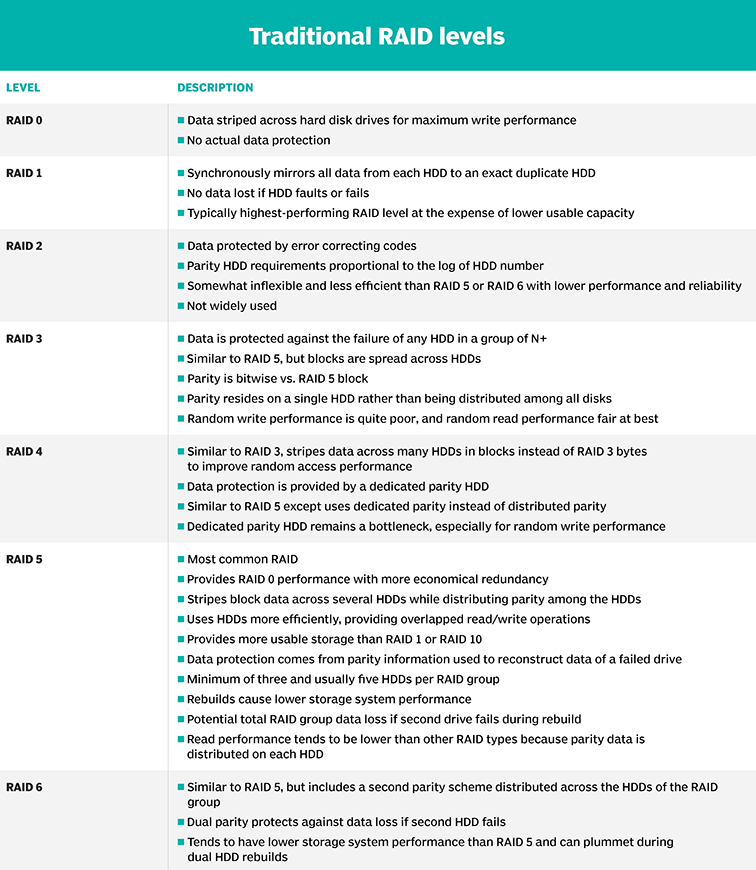
\includegraphics[width=\textwidth]{storage_raid_levels}
%	\caption{Traditional RAID Levels}\label{fig_raid_table}
%\end{figure}

%Look ahead buffer
%Look aside buffer

%Reread Questions:
%Disks: GATE1997-74
%Disks: GATE2004-49
%User level-threads, kernel supported threads